\chapter{Ръководство на потребителя}
\section{Инсталация}
\subsection{Изтегляне}
Spellbook е достъпен за изтегляне под формата на пакети за Red Hat и
Debian базирани GNU/Linux дистрибуции, инсталатор за Windows и
платформено независим архив.

Всички те са достъпни на официалния сайт на проекта
\textbf{http://code.google.com/p/spellbook-dictionary/}. Там също така
е достъпна за сваляне речниковата база данни. Текущото ръководство е
достъпно в HTML формат.
\subsection{Инсталация}
\begin{itemize}
  \item \textbf{Инсталация под Red Hat GNU/Linux}

    Изтеглете файла spellbook-0.3.0-1.noarch.rpm. Инсталирайте файла с
    командата:

    \textbf{sudo rpm -Uhv spellbook-0.3.0-1.noarch.rpm}

    Spellbook се нуждае от Java 6 за да работи. Ако нямате инсталирана
    Java инсталирайте OpenJDK или Sun JRE. OpenJDK може да бъде
    инсталирано с командата:

    \textbf{sudo yum install java-1.6.0-openjdk java-1.6.0-openjdk-plugin}

    Sun Java може да изтеглите от
    http://java.sun.com/javase/downloads/index.jsp. 

    За предпочитане е да използвате Sun Java, тъй като проблемите в
    нея се отстраняват по-бързо от разработчиците.
   
    \item \textbf{Инсталация под Debian GNU/Linux}

      Изтеглете файла spellbook-0.3.0-1.noarch.deb. Инсталирайте файла с
    командата:

    \textbf{sudo dpkg -i spellbook-0.3.0-1.noarch.deb}

    Spellbook се нуждае от Java 6 за да работи. Ако нямате инсталирана
    Java инсталирайте OpenJDK или Sun JRE. OpenJDK може да бъде
    инсталирано с командата:

    \textbf{sudo apt-get install java-1.6.0-openjdk java-1.6.0-openjdk-plugin}

    Sun Java може да изтеглите от
    http://java.sun.com/javase/downloads/index.jsp. 

    За предпочитане е да използвате Sun Java, тъй като проблемите в
    нея се отстраняват по-бързо от разработчиците.

    \item \textbf{Инсталация под Windows}

      Изтеглете файла spellbook-0.3.0-1-installer.exe. Инсталирайте
      файла като кликнете два пъти върху него.

    Spellbook се нуждае от Java 6 за да работи. Sun Java може да изтеглите от
    http://java.sun.com/javase/downloads/index.jsp. 

    \item \textbf{Инсталация на платформено независимия архив}

      Изтеглете файла spellbook-0.3.0-1.tar.bz2. Разархивирайте файла с
    командата:

    \textbf{tar xf spellbook-0.3.0-1.tar.bz2}

    или с графична програма за работа с архиви. След това влезте в
    директорията, която се появява след разархивирането на файла. Ако
    използвате Unix базира операционна система стартирайте файла
    spellbook, ако използвате Windows система - кликнете два пъти
    върху файла spellbook-0.3.jar

    Spellbook се нуждае от Java 6 за да работи. Ако нямате инсталирана
    Java инсталирайте OpenJDK или Sun JRE. Инсталирайте ги по
    предпочитания от вас начин съвместим с използваната от вас
    операционна система.

    Sun Java може да изтеглите от
    http://java.sun.com/javase/downloads/index.jsp. 

    За предпочитане е да използвате Sun Java, тъй като проблемите в
    нея се отстраняват по-бързо от разработчиците.
\end{itemize}
\section{Известни проблеми}
Въпреки огромното старание, което се полага за да работи Spellbook
еднакво добре навсякъде, това не винаги е възможно. Ето списък с
известни проблеми, остраняването, на които не зависи от автора.
\begin{itemize}
  \item Когато се ползва OpenJDK не е достъпен външният вид Nimbus,
    тъй като той още не е включен там
  \item Когато се ползва OpenJDK не е достъпна трей инонката, ако
    ползвате десктоп мениджър различен от Metacity.
\end{itemize}
За да са наясно потребителите с тези проблеми при стартирането си
приложението засича върху каква виртуална машина е пуснато и
предупреждава потребителя, ако тя не е препоръчваната Sun HotSpot VM.
\begin{figure}[htbp]
  \caption{Предупреждение за несъвместима виртуална машина}
  \centering
  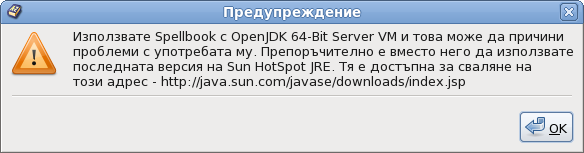
\includegraphics[width=110mm, height=40mm]{images/jre_warning.png}
\end{figure}
\section{Стартиране}
Стартирането на Spellbook е напълно стандартно - може да го стартиране
от неговия изпълним файл spellbook под Unix подобна операционна
система, от неговата секция в старт менюто на вашата система или от
самият jar архив на програмата. Ако сте асоциирали програмата Java с
типа jar кликването два пъти върху файла ще го стартира. Алтернативата
е командата:

\textbf{java -jar spellbook-0.3.jar}

Системата показва специален екран на зареждане(splashscreen), на който
се отчита докъде е достигнал процеса на зареждане. Той изглежда по
следния начин:

\begin{figure}[htbp]
  \caption{Екран на зареждане}
  \centering
  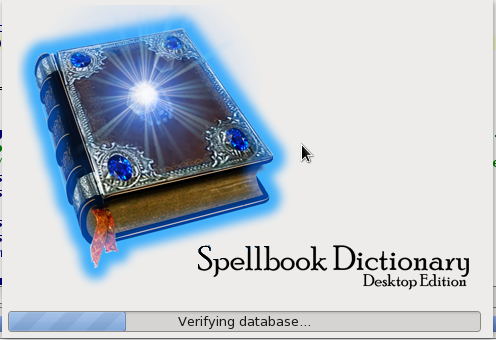
\includegraphics[width=90mm, height=80mm]{images/splashscreen.png}
\end{figure}

Трябва да имате в предвид, че в един момент може да имате само една
инстанция на Spellbook, която да работи. Ако се опитате да стартирате
нова инстация, докато работи друга ще бъдете предупредени със
съобщение. След като потвърдите съобщението инстанцията, която се
опитвате да стартирате ще преустанови работата си. Това ограничение се
налага главно от модела на работата на вградените бази данни(каквото
използва Spellbook за вътрешно съхраниение на информацията) - при тях
само един процес може да достъпва в даден модел базата данни. Имайте в
предвид, че този процес може да не е Spellbook въобще - ако използвате
някоя програма за администрация на бази данни или какъвто и да е било
клиент на базата данни, това ще я направи недостъпна за всяко друго
приложение и ще получите гореспоманата грешка.

\begin{figure}[htbp]
  \caption{Съобщение за наличение на друга работеща инстанции}
  \centering
  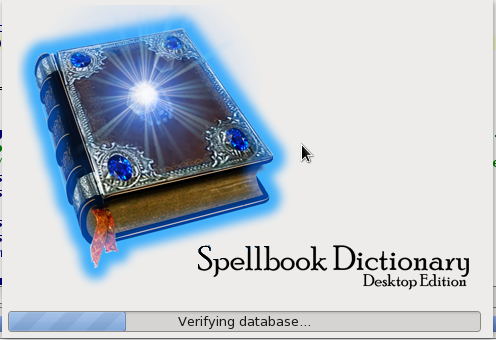
\includegraphics[width=90mm, height=80mm]{images/splashscreen.png}
\end{figure}

Първото стартиране на Spellbook е специално. Ще ви бъде показа
диалогов прозорец, от който може да изтеглите речниковата база данни
на Spellbook автоматично от интернет или да укажете пътя до нея, ако
сте я свалили отделно(това не важи за случая, в който сте използвали
Windows инсталаторът, тъй като актуалната версия на базата данни е
пакетирана направо в него).
\begin{figure}[htbp]
  \caption{Диалогов прозорец за избор на база данни}
  \centering
  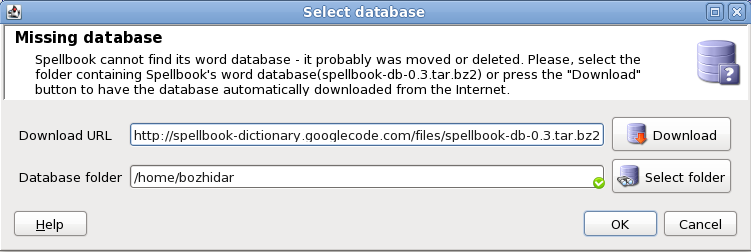
\includegraphics[width=110mm, height=40mm]{images/select_db.png}
\end{figure}

След като изтеглите речниковата база данни или укажете пътя до нея в
локалната файлова система тя ще бъде автоматично декомпресирана и
разархивирана и Spellbook ще ви покаже своя речников изглед.

Системата по подразбиране ще стартира с потребителски интерфейс на
английски език. Целият интерфейс, обаче, е преведен и на
български. Ако предпочитате българският интефейс, просто го задайте
като език по подразбиране в настройките на приложението.

В случай, че сте избрали настройката "`Проверка за нова версия при
стартиране"' и такава е налична ще бъдете уведомени за това с диалогов
прозорец.

\begin{figure}[htbp]
  \caption{Диалогов прозорец за наличение на нова версия}
  \centering
  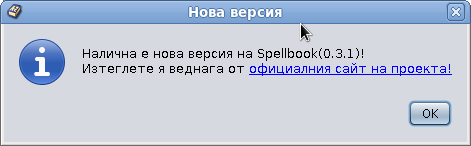
\includegraphics[width=110mm, height=40mm]{images/new-version.png}
\end{figure}

Новите версии винаги са достъпни за сваляне от секцията Downloads на
официалния сайт. В бъдеще вероятно ще бъде включена възможност за
авматично обновяване на приложението до последната му версия.
\section{Речник}
Речниковият изглед на Spellbook е изгледът, който ще видите веднага
след зареждането на програмата. Ще бъде зареден речникът по
подразбиране(който се указва в настройките на приложението) и вие
веднага може да започнете да правите речникови справки. В зависимост
от това дали е избрана опцията "`Дума на деня"' при стартиране на
системата ще ви бъде показана прозволна дума от речника по подразбиране.
\begin{figure}[htbp]
  \caption{Дума на деня}
  \centering
  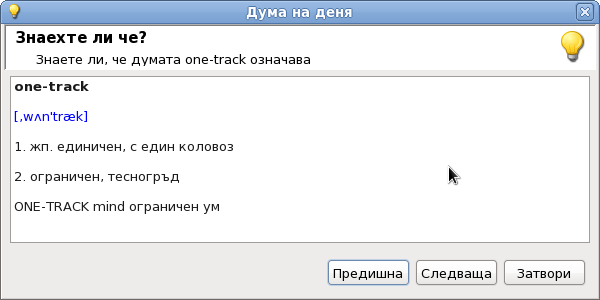
\includegraphics[width=110mm, height=40mm]{images/word_of_the_day.png}
\end{figure}

Речниковата перспектива има няколко части - лента с менюта, лента с
бутони(toolbar) и самият речников изглед, разбира се. Посредством
менютата и бутоните могат да бъдат достъпени всички други елементи на системата.
\begin{figure}[htbp]
  \caption{Главен речников изглед}
  \centering
  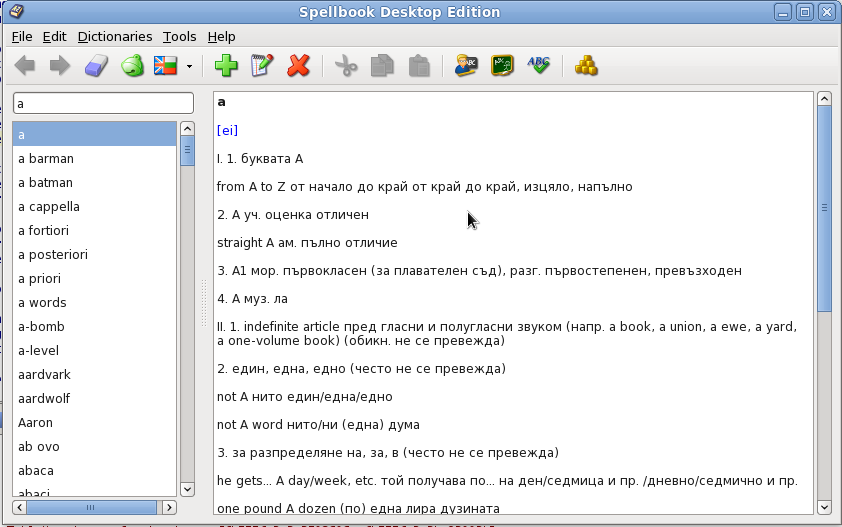
\includegraphics[width=110mm, height=70mm]{images/dictionary_view.png}
\end{figure}

Търсенето на дума в речника е много лесно - просто започнете да пишете
думата в полето за търсене и на всеки натискат от вас клавиш ще ви
бъде показвана, думата най-близо до вашето търсене или евентуално
точно попадение, ако същестува такова. Когато намерите думата, която
търсите натиснете клавиша "`Enter"', за да запазите намерената дума в
историята на Spellbook и да я селектирате за да може да бъде изтрита
лесно с натискането на един клавиш(Backspace). Spellbook е проектиран
така, че работата в него да бъде удобна както за хора предпочитащи да
работят с мишка, така и за тези предпочитащи да работят с клавиатура.

По всяко време може да изтриете текущата дума и с бутона "`Изтрий"'
или да запазите думата в историята с бутона "`Запази в
историята"'. Между думите в историята може да навигирате с двата
бутона стрелки в началото на лентата с бутоните. Освен това, освен
тогава, ако започнете да въвеждате нова дума в полето за търсене,
която започва по същия начин, като дума запазена в историята ще видите
списък с предложения за дописване(autocompletion), които може веднага
да селектирате с клавиатурата или мишката.

Spellbook е организиран върху идеята за комплементарни
речници(наричани в друга литература двустранни). Ако избраният от вас
в момента речник е комплементарен - например Анлийско-Български и ако
е избран от него анлийско-българския речник в момента, а вие искате да
търсите превода на българска дума на анлийски, не е необходимо да
превключвате ръчно речниците. Започнете да пише думата на български и
Spellbook автоматично ще превключи към другата половина на
комплементарния речник. Превключването между комплементарните речници
е достъпно и посредством бутона с иконка речник в лентата с
бутони. Всички речници са достъпни за избор, както от падащото меню
асоциирано с този бутон, така и посредством менюто "`Речници"' в
лентата с менюта на приложението.

Ако сте активирали опциите "`Интеграция с клипборда"' и "`Показване на
балони с преводи"' дори няма нужда да пишете думата, която искате в
Spellbook. Маркирайте я и я копирайте в системния clipboard(например с
клавишната комбинация Control + C) - Spellbook ще отчете това и ще ви
покаже превода и автоматично.

В речниковият режим, разбира се, са достъпни команди за манипулация на
текст от общо ниво като "`копирай"', "`изрежи"', "`пренеси"'. Те са
достъпни от менюто на приложението, от лентата с бутоните и като
контекстно меню(меню, което се появява, като натиснете десният бутон
на мишката).
\section{Изпит}
Изпитът може да бъде достъпен от менюто "`Инструменти"' или от лентата
с бутони. По същество изпитът представява превод на думи от един език
на друг. Може да бъде провеждан изпит на всеки език, за който
Spellbook разполага с комплементарен речник. 

\begin{figure}[htbp]
  \caption{Изпит}
  \centering
  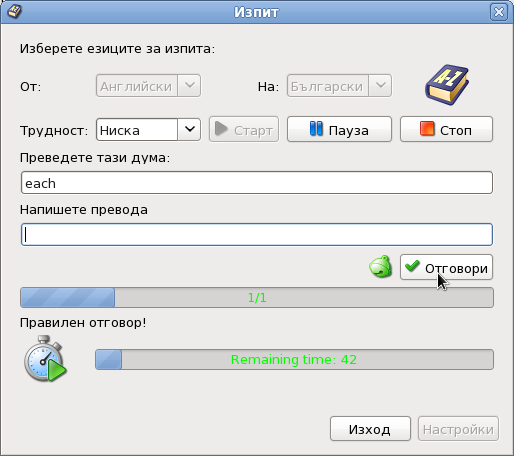
\includegraphics[width=110mm, height=70mm]{images/exam_dialog.png}
\end{figure}

Преди започване на изпита потребителя трябва да избере езика, от който
иска да превежда, езика, на който да превежда и трудността на
изпита. Натискането на бутона "`Старт"' стартира изпита. Изпита може
да бъде спрян временно с бутона "`Пауза"' или прекратен преждевременно
с бутона "`Стоп"'. 

При приключването на изпита ще ви бъде показан екран с обща информация
за представянето ви. За да вземете изпит успешно трябва да отговорите
правилно на поне 60 процента от въпросите в изпита. Оценките са както
следва:
\begin{itemize}
  \item \textbf{Слаб} - резултат 0-59
  \item \textbf{Среден} - резултат 60-69
  \item \textbf{Добър} - резултат 70-79
  \item \textbf{Много добър} - резултат 80-89
  \item \textbf{Отличен} - резултат 90-100
\end{itemize}

Освен това имате възможност да запишете вашият резултат и да
прегледате сгрешените от вас думи. 
\section{Учене на думи}
Модулът "`Учене на думи"' ви дава възможност да създадете набор от
думите, които представляват интерес за вас - например думите от
последния урок на езиковия курс, който посещавате, или думите, които
могат да се паднат на изпита САТ1. След това имате възможност да
провеждате "`локализиран изпит"' върху тези думи, като имате
възможност да настройвате реда на показването им и други атрибути.

\begin{figure}[htbp]
  \caption{Учене на думи}
  \centering
  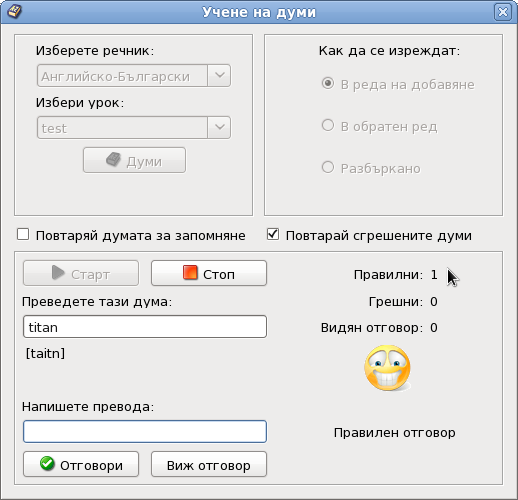
\includegraphics[width=110mm, height=70mm]{images/study_words.png}
\end{figure}

Наборите от думи могат да се запазват да ги използвате по-късно
отново.

\begin{figure}[htbp]
  \caption{Добавяне на думи в набор за учене}
  \centering
  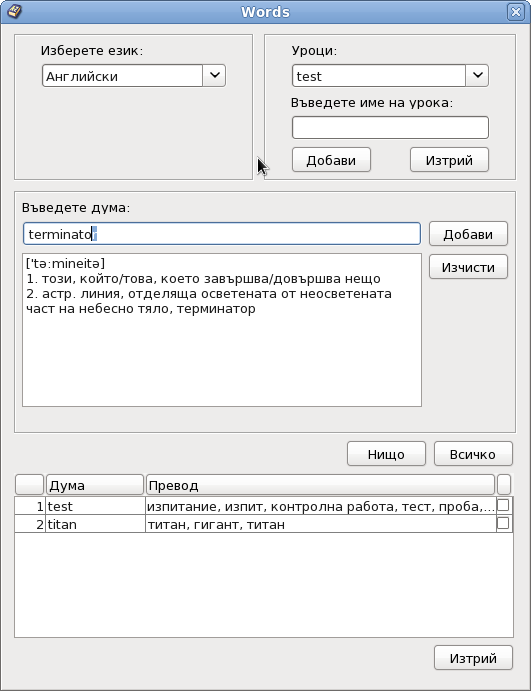
\includegraphics[width=110mm, height=70mm]{images/add_to_study_set.png}
\end{figure}

\section{Проверка на правопис}
Проверката на правописа може да бъде стартирана от менюто
"`Инструменти"' или от лентата с бутони. Използването и е лесно и
интуитивно - избирате език, копирате текста, който искате да бъде
проверен и грешните думи веднага ще бъдат подчертани. Когато кликнете
с дясното копче върху сгрешена дума ще получите предложения за нейната
корекция. 

\begin{figure}[htbp]
  \caption{Проверка на правописа}
  \centering
  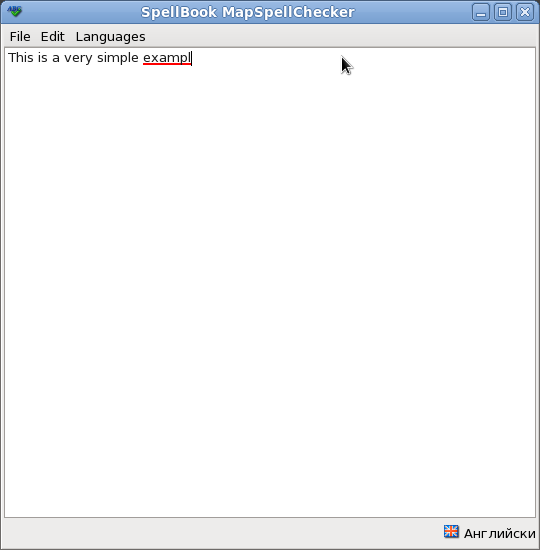
\includegraphics[width=110mm, height=70mm]{images/spellcheck_frame.png}
\end{figure}

Имате и възможност да добавяте думи в речника на инструмента.
\section{Настройки}
Много аспекти на Spellbook подлежат на конфигурация от страна на
потребителя. Настройките са достъпни посредством менюто
Редактирай->Настройки(Edit->Preferences). Групирани са в три по-общи
категории - общи настройките, които касаят повече от един аспект от
работата на системата, настройки на шрифтовете и настройки на
изпита. В бъдеще броят на секциите вероятно ще бъде увеличен, тъй като
възможността за персонализиране на максимален брой от възможностите на
едно приложение е ключова.
\subsection{Общи}
\begin{figure}[htbp]
  \caption{Общи настройки}
  \centering
  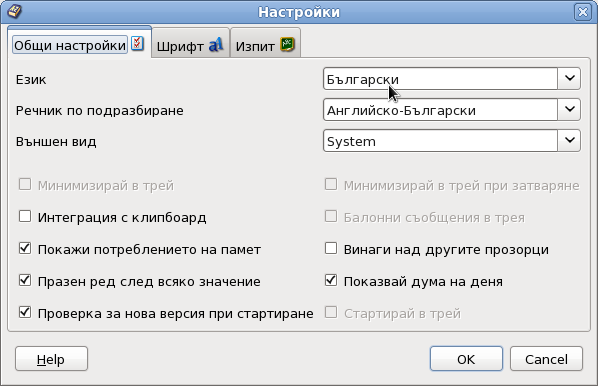
\includegraphics[width=110mm, height=70mm]{images/general_preferences.png}
\end{figure}

Кратко описание на настройките налични в тази секция:
\begin{itemize}
  \item \textbf{Език}

    Езикът на потребителския интерфейс. Възможните стойности са две -
    \emph{Български} и \emph{Английски}. Променята на стойността на тази настройка
    \emph{изисква да рестартирате} Spellbook. 
  \item \textbf{Речник по подразбиране}

    Речникът, който да се зарежда по подразбиране от
    приложението. Броят на възможностите, които виждате зависи от
    версията на базата данни, която използвате.
  \item \textbf{Външен вид}

    Външният вид на приложението. Настойките, които виждате тук
    зависят от вашата операционна система - например потребителите на
    Windows ще виждат външен вид Windows, а тези на Linux - GTK+. За
    всяка операционна един външен вид е маркиран като външен вид по
    подразбиране - за Unix базираните операционни системи това е GTK+,
    за Windows системите - това е или Windows Classic или Windows. 
    Външния видове като Metal и Nimbus са платформено независими и са
    достъпни винаги. Nimbus е достъпен във версии на Sun Java по-нови
    от 1.6.10, но все още не е достъпен в OpenJDK. Nimbus е външният
    вид по подразбиране на Java(Metal беше старият външен вид по
    подразбиране). Spellbook селектира по подразбиране въшния вид
    считан за външен вид по подразбиране на операционната система,
    която използвате. 
  \item \textbf{Минимизирай в трей}
    
    Когато тази настройка е избрана Spellbook ще се скрива в областта
    за уведомяване(system tray), вместо на обичайното си място. За да
    го възстановите трябва да кликнете неговата икона в областта на
    уведомяване. Не винаги е възможно да изберете тази опция - тя е
    деактивирана за десктоп мениджъри, за които няма поддръжка на
    областта за уведомяване в Java.
  \item \textbf{Минимизирай в трей при затваряне} 

    Когато тази настройка е избрана Spellbook ще се скрива в областта
    за уведомяване(system tray) при затваряне, вместо да прекрати
    работата си. За да го възстановите трябва да кликнете неговата
    икона в областта на уведомяване. Не винаги е възможно да изберете
    тази опция - тя е деактивирана за десктоп мениджъри, за които няма
    поддръжка на областта за уведомяване в Java.

  \item \textbf{Интеграция с клипборд}
    
    Когато тази настройка е активна думите, които копирате в системния
    клипборд ще бъдат превеждани автоматично от Spellbook. Когато
    копирате повече от една дума само първата ще бъде преведена. Ако
    не бъде открито точно съвпадение ще си бъде показано най-близкото
    попадение. Ако се налага Spellbook ще превлючи автоматично към
    комплементарен речник. Интеграцията с клипборда може да ви създаде
    проблеми с други приложения, тъй като поради ограничения на Java
    се налага Spellbook да възприема постоянно собствеността на
    клипборда. Това обикновено не е проблем, но ще е проблем, ако
    някоя друга програма зависи от същото поведение за нормалната си
    работа. 
  \item \textbf{Балонни съобщения в трей} 

    Разширение на интеграцията с клипборд. Ако е селектирано преводът
    на думите бива показан в съобщение в областта за нотификация. Ако
    го кликнете ще бъде отворена главната(речникова) перспектива на
    Spellbook. Съобщението изчезва само след няколко секунди. Не
    винаги е възможно да изберете тази опция - тя е деактивирана за
    десктоп мениджъри, за които няма поддръжка на областта за
    уведомяване в Java.
  \item \textbf{Покажи потреблението на памет}

    Когато тази опция е избрана в лентата с бутони на приложението се
    появява допълнителен бутон. Задържането на курсора на мишката над
    него показва потреблението на памет от приложението, а натискането
    му форсира събирането на боклука на Java виртуалната машина. 
  \item \textbf{Винаги над другите прозорци}

    Името на тази опция е доста самоописалено - когато тя е избрана
    Spellbook ще бъде винаги над прозорците на другите приложения на
    десктопа, независимо дали има фокус или не в момента.
  \item \textbf{Празен ред след всяко значение}

    Когато тази опция е избрана във форматирането на преводите на
    думите се добавя допълнителен ред след всяко значение на дума, с
    цел да се подобри четимостта им.
  \item \textbf{Показвай дума на деня}

    Когато тази опция е избрана при стартирането на Spellbook бива
    показана произволна дума от речника по подразбиране.
  \item \textbf{Проверка за нова версия при стартиране}

    Когато тази опция е избрана Spellbook проверява автоматично за
    наличието на нова версия и уведобавя потребителя, в случай че
    такава наистина съществува.
  \item \textbf{Стартирай в трей}
    
    Когато тази опция е избрана приложението ще стартира скрито в
    областта за уведомяване. Не винаги е възможно да изберете тази
    опция - тя е деактивирана за десктоп мениджъри, за които няма
    поддръжка на областта за уведомяване в Java.
  \item \textbf{Игнорирай проблеми със съвместимостта}

    Когато тази опция е избрана бива потиснато съобщението за
    потенциални проблеми в съвместимостта на използваната от
    потребителя версия на Java и Spellbook. За справка вижте секцията
    "`Известни проблеми"'.
\end{itemize}
\subsection{Шрифтове}
В секцията посветена на шрифтовете може да изберете следните атрибути
на шрифта, използван в приложението:

\begin{itemize}
  \item \textbf{Име на шрифта}

    Шрифтовете, които ще видите тук зависят както от вашата
    операционна система, така и от приложенията/пакетите, които сте
    инсталирали до момента. Важно е да изберете подходящ шрифт, който
    да възпроизвежда правилно символите от езиците, с които планирате
    да работите.
  \item \textbf{Стил на шрифта}

    Стила на шрифта може да бъде нормален или комбинация от удебелен,
    подчертан и курсив.
  \item \textbf{Размер на шрифта}

    Размерът на шрифта в точки(points). 
\end{itemize}

Промените, които правите в тези настройки моментално се отразят на
полето "`Преглед"'. Така имате предварително идея, дали избраните от
вас настройки биха ви допаднали.

\begin{figure}[htbp]
  \caption{Главен речников изглед}
  \centering
  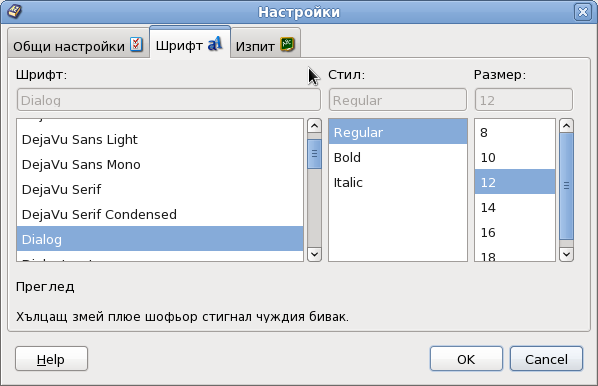
\includegraphics[width=110mm, height=70mm]{images/font_preferences.png}
\end{figure}

\subsection{Изпит}

В тази секция може да конфигурирате някои аспекти от поведението на
изпита, а именно:

\begin{itemize}
  \item \textbf{Трудност по подразбиране}

    Трудността по подразбиране на изпита. Възможните стойности са
    "`Ниска"', "`Средна"' и "`Висока"'. Трудностите за всеки език се
    определят посредством статистически анализ на език, т.е. на
    по-високи трудности ще срещате по-рядко срещани в езика думи.

  \item \textbf{Дължина на изпита}

    Дължината на изпита в брой думи.

  \item \textbf{Изпит с време}

    По принцип изпита няма време, т.е. имате неограничен период от
    време да отговорите на някой въпрос. Ако активирате тази
    настройка, обаче, това ще се промени. Ще виждате визуален таймер,
    който показва колко време ви остава за отговор. Ако таймера изтече
    преди да дадете отговор - въпросът се счита за сгрешен. В
    нарастване на трудността на изпита време за отговор намалява. За
    ниска трудност то е 45 секунди, за средна - 30, а за висока - само
    15.
\end{itemize}

\begin{figure}[htbp]
  \caption{Настройки на изпит}
  \centering
  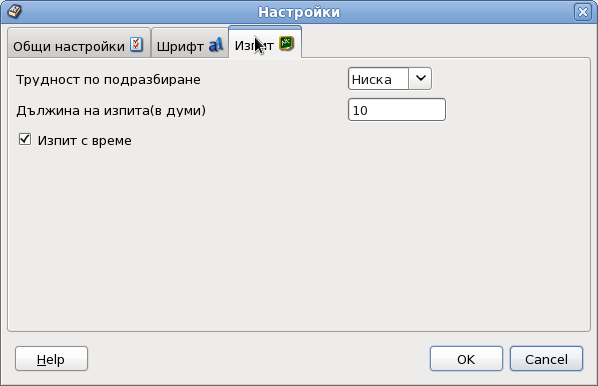
\includegraphics[width=110mm, height=70mm]{images/exam_preferences.png}
\end{figure}

\section{Манипулиране на речниковата база}
За разлика от много други подобни приложения Spellbook позволява на
потребителите да редактират речникова база данни. Операциите, които те
могат да извършват върху нея са добавяне на нови думи, редактиране на
съществуващи думи и изтруване на думи.

Диалога за манипулация на думи може да бъде извикан от менюто
"`Редактирай"' или от лентата с бутони. Операциите "`Редактирай"' и
"`Изтрий"' са активни само, ако е избрана дума в списъка с думи на
текущия речник. Допълнително "`Редактирай"' може да се активира и
просто като щракнете с левия бутон на мишката два пъти върху дума в
списъка с думи. 

\begin{figure}[htbp]
  \caption{Настройки на изпит}
  \centering
  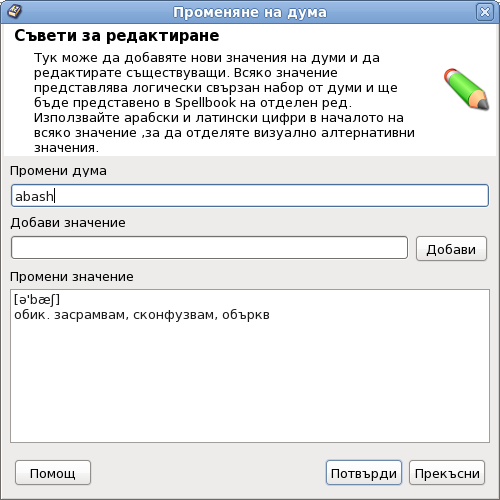
\includegraphics[width=110mm, height=70mm]{images/edit_word.png}
\end{figure}

Локално направените от вас промени по речниковата база данни в
последствие могат да бъдат синхронизирани с централната база данни на
Spellbook. Така от промените направени от вас печели цялата
потребителска общност.
\section{Персонализиране на външния вид}
В менюто "`Изглед"' ще откриете няколко настройки, чрез които може да
персонализирате външния вид на приложението по ваш вкус. По настоящем
са възможни следните действия:

\begin{itemize}
  \item Показване/скриване на лентата с бутоните за бърз достъп.

    Когато размаркирате тази отметка лентата с бутони на приложението
    моментално ще изчезне. Лентата с бутони е видима по
    подразбиране. Настройките въведени в това меню се запазват
    автоматично за бъдещи стартирания на програмата.

    \item Показване/скриване на статус лентата

      Когато размаркирате тази отметка лентата със статуса на приложението
    моментално ще изчезне. Лентата със статуса е видима по
    подразбиране. Настройките въведени в това меню се запазват
    автоматично за бъдещи стартирания на програмата.

\end{itemize}

Въпреки, че Spellbook е напълно използваем без двете гореспоменати
ленти в тях потребителите имат достъп до полезна информация и
възможности и затова им се пропоръчва да оставят поне едната от тях видима.

\section{Помощ}

В секцията "`Помощ"' на приложението може да откриете неговата
документация, както и информация за лиценза и екипа на проекта, както
и връзка към официалния му сайт. Проектът е лицензиран под свободния
лиценз GNU General Public License Version 3. Пълният текст на лиценза
е достъпен, като натиснете бутона "`Лиценз"' в диалоговия прозорец
"`Относно"'.

\begin{figure}[htbp]
  \caption{Настройки на изпит}
  \centering
  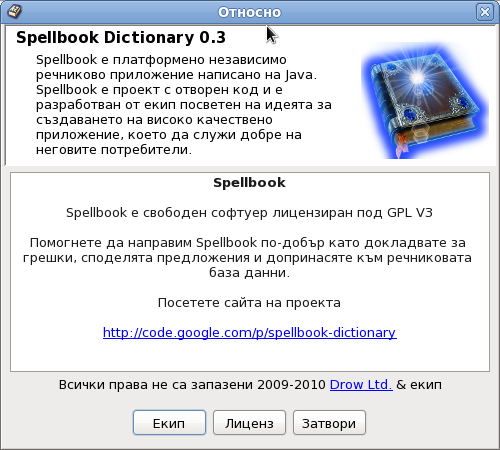
\includegraphics[width=110mm, height=70mm]{images/about_dialog.png}
\end{figure}

Освен това може да проверите за наличнието на нова версия като
изберете "`Проверка за нова версия"' в менюто "`Помощ"'. В зависимост
от нова, дали е налична или не нова версия ще видите един от тези два
диалогови прозореца.

\begin{figure}[htbp]
  \caption{Нова версия}
  \centering
  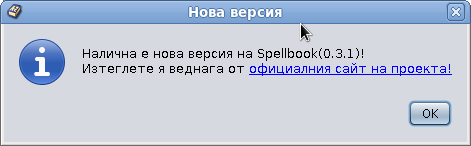
\includegraphics[width=110mm, height=40mm]{images/new-version.png}
\end{figure}


\begin{figure}[htbp]
  \caption{Няма нова версия}
  \centering
  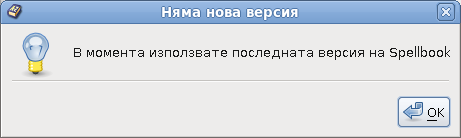
\includegraphics[width=110mm, height=40mm]{images/no-new-version.png}
\end{figure}

В менюто "`Помощ"' има възможност и да докладвате за проблем, с който
сте се сблъскали, докато сте използвали Spellbook. Това става като
селектирате "`Докладвай грешка"'. Ще ви бъде представен диалогов
прозорец, в който да въведе кратно описание на проблема(заглавие) и
после малко по-подробно да го опишета като включите например съобщение
за грешка, което сте получили или пък стъпки за възпроизвеждане на
проблема. Информация за средата на изпълнение - версия на Java,
операционна системата също са много полезни. 

\begin{figure}[htbp]
  \caption{Диалогов прозорец за докладване на грешка}
  \centering
  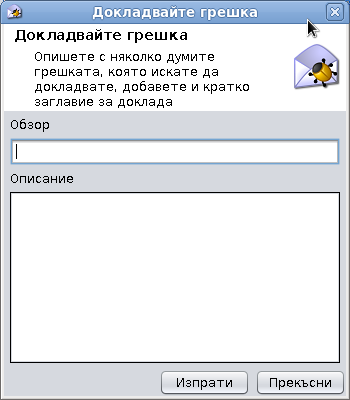
\includegraphics[width=90mm, height=70mm]{images/report-bug.png}
\end{figure}

Когато натиснете бутона изпрати ще бъде създаден доклад за грешка в
системата за следене на грешки на приложението и той ще бъде възложен
на някой от разработчиците на Spellbook, който ще се постарае да
отстрани проблема максимално бързо.
 
%%% Local Variables: 
%%% mode: latex
%%% TeX-master: "master"
%%% End: 
